\documentclass[12pt]{article}
\usepackage{graphicx}
\usepackage{amsmath}

\usepackage[hidelinks]{hyperref}
\hypersetup{
    colorlinks=true,
    linkcolor=blue,
    filecolor=magenta,      
    urlcolor=cyan,
}

\hyphenation{Model-Sim}

\begin{document}

\title{LEG Processor for Education\\\Large{System Documentation}
}
\author{TODO: authors or contact}
\date{Last Modified \today}
\maketitle
\thispagestyle{empty}
\pagebreak
\setcounter{page}{1}
\pagebreak

\tableofcontents
\pagebreak

\section{TODO}
\begin{itemize}
\item Copyright signs on programs? (e.g. ModelSim)
\item Change repository link to public version and verify installation
\item How to get linux? Include in repository?
\end{itemize}

\section{Getting Started}
LEG processor development begins by downloading the code base to your local machine or a shared class drive.
The code base is small enough for each user to have a local copy.
After cloning the LEG repository, only a few off the shelf programs are required to get the processor running.
Complete instructions are presented here for Linux systems, but most functionality is available on Windows.

Several programs must be installed to use the full LEG debugger. 
However, only the LEG repository must be downloaded if you are only interested in examining the source files.

\begin{enumerate}
\item Install git if it is not already installed, and clone the LEG git repository from \url{https://github.com/EStorm21/LEG.git}
\item Install the free Starter Edition of ModelSim from \url{http://dl.altera.com} or any version of ModelSim you may already have purchased. Note that in Starter Edition performance will be reduced and some features such as checkpoints will be unavailable. LEG has been tested on ModelSim version SE 10.3d. 
\item Ensure that GDB is installed on your system. Download it from \url{https://www.gnu.org/software/gdb/download/} or through your package manager.
\item Install QEMU from \url{http://wiki.qemu.org/Download}. (or from package manager?)
\item Modify configuration files to point to your installation of stuff?
\end{enumerate}



\section{Basic Testing}
\section{Testing}

\subsection{Brief Overview}
This section describes the procedure for generating and running tests. 


\subsection{All Relevant Files and Brief Descriptions}
\begin{itemize}
\item \textbf{makeQemuTest.sh} Creates testing files from an assembly source. Results are derived from QEMU. 
\item \textbf{testManual.sh} Allows the user to single-step assembly in QEMU. 
\item \textbf{autosim0.tcl} Runs the tests in tests.list against ModelSim. 
\item \textbf{autoSim1.tcl} Opens a single test in ModelSim with the GUI. 
\item \textbf{makePiTest.sh} Creates testing files from an assembly source. Results are derived from the raspberry pi. 
\end{itemize}

\subsection{Creating Tests}
There are two methods for creating tests, either on tera, verified by QEMU, or on the raspberry pi, verified by GDB on the pi. Both methods currently depend on the Pi for assembly and disassembly. 
\subsubsection{Creating Tests on Tera}
Tests can be created on tera in \texttt{/proj/leg/qemu}. 
First create an assembly file of instructions to test. 
This test should have appropriate exception handling setup with branches in the base addresses to each exception handler. 
The results are compared to the integrator board in QEMU. 
The bootloader in QEMU initializes the flags and puts values in r0 and r1. 
To ensure consistent results when comparing ModelSim and QEMU, all tests should start by setting r0, r1, and the condition flags. 
All assembly files should have a \texttt{.s} file extension, for example \texttt{add.s}. To generate the test files, use \texttt{makeQemuTest.sh}. 
For example \texttt{sh makeQemuTest.sh add}

Once the script is started, it will transfer several files to and from the Pi. If you intend to create a lot of tests, you should create a public key for the pi so you don't have to keep typing in the password. Once the files have transferred, QEMU will start. To get the results from QEMU type \texttt{info registers} the \texttt{Ctrl+C} to quit QEMU. This will create the test. 

The results of this process leave you with 6 files. 
\begin{itemize}
\item \texttt{.bin} file: The binary file which can be run on the Pi for debugging. 
\item \texttt{.dat} file: The file that runs on ModelSim. 
\item \texttt{.dump} file: The objdump file that contains useful human readable information about the test.
\item \texttt{.flash} file: The QEMU readable file. 
\item \texttt{.s} file: The assembly source file.
\item \texttt{.val} file: The state of the registers at the end of the program, for comparison against ModelSim. 
\end{itemize}

\subsubsection{Creating Tests on the Pi}
Test creation on the Pi is analagous to tera. 
The username and password for the pi are pi and strawberry, respectively. Creating tests on the Pi does not generate the QEMU compatible file. Generating tests on the pi does not accomodate mode changes and all instructions are executed in user mode. 
\subsection{Running Tests}

Running tests requires modification of the default \texttt{autoSim0.tcl} 
file in the project root directory (assumed in this document to be \texttt{/LEG} )
and the \texttt{dmem.sv} file in \texttt{LEG/leg\_pipelined/dmem.sv}. 
Note that the path after \texttt{/LEG} is shown, but absolute paths are 
required for all files and directories.

\subsubsection{Modifying \texttt{autoSim0.tcl}}

\begin{enumerate}
	\item Create an empty ModelSim project in your favorite directory.
	\item Create an unversioned copy of \texttt{autoSim0.tcl} for your own use.
	\item Modify the entries in the copy to point to the correct locations:
	\begin{itemize}
		\item \texttt{project} should point to your ModelSim project.
		\item On your own computer, \texttt{vlog} should end in \texttt{LEG/leg\_pipelined/*.sv}
		\item \texttt{testPath} should point to \texttt{LEG/tests}
		\item \texttt{testList} should point to \texttt{LEG/tests/tests.list}
		\item In the test for loop, change the location of simTest.dat to a directory 
		of your choice, e.g. \texttt{LEG/tests/simTest.dat}
	\end{itemize}
\end{enumerate}

\subsubsection{Modifying \texttt{dmem.sv}}

\begin{enumerate}

\item Comment out the other \texttt{\$readmemh} lines, and add your own with 
the same path to the \texttt{simTest.dat} file. Each time you pull from 
the repository and want to run tests you will need to uncomment 
the correct line in this file. Alternatively, don't commit this file.

\item In most cases you can also comment out the loop that fills the memory with zeros. 
This will cause the tests to run faster.
\end{enumerate}


\subsubsection{Run tests and view output}

\begin{enumerate}
	\item Uncomment the test you want to run in \texttt{LEG/tests/tests.list}.
	\item Using a shell (Cygwin, PowerShell, cmd on Windows), 
	navigate to the folder containing your \texttt{autosim.tcl} file. 
	\item run the command \texttt{vsim -c -do autosim.tcl}
	\item One way to view in ModelSim on your computer is to use the autoSim1.tcl file
	(modified for your setup). Run this in command prompt and ModelSim will open. Add waves and restart.
\end{enumerate}

\subsubsection{autosim1.tcl}
autosim1.tcl is a script on tera for manually debugging a single test. 
The test is loaded into dmem.sv, and the GUI is loaded. 
The user can then add additional signals and quickly restart the simulation. 

\pagebreak

\section{Advanced Testing and Simulator Operation}
% TODO
\section{debug\_lockstep}

\subsection{Brief Overview}

This is a tool I made to enable fast debugging and testing of the Linux kernel by comparing the registers of qemu with those of the LEG processor simulated in ModelSim.

\subsection{All Relevant Files and Brief Descriptions}

\begin{itemize}
\item \textbf{checkpoint.py} Python file that handles creation of checkpoints.
\item \textbf{checkpoint.tcl} Simple tcl file to create a checkpoint.
\item \textbf{debug.py} Python file that is executed within GDB and sets up the debugging commands.
\item \textbf{debug.sh} Script to start the debugging process.
\item \textbf{debug.tcl} Tcl script that handles lockstep debugging on the ModelSim end.
\item \textbf{lockstep.py} Python file that handles lockstep debugging on the GDB end.
\item \textbf{qemuDump.py} Python file that handles dumping Qemu's current state to file.
\item \textbf{qemuDumpRestore.tcl} Tcl script that manipulates the ModelSim state to match a dumped Qemu state.
\end{itemize}

\subsection{File structure}
The run directory on Tera is currently in the Git repo at \texttt{debug\_lockstep}.1 The scripts place all of their output in the \texttt{debug\_lockstep/output} directory. For each run of the script, a new subdirectory within this directory is created, named according to the appropriate timestamp. Within this directory, the \texttt{bugs} directory contains the full debug output of each found bug, and \texttt{runlog} contains an abbreviated summary of all bugs found in the given run. Duplicate bugs are ignored and do not appear in these files.

Created checkpoints appear in \texttt{output/checkpoints/} with the provided name.

\subsection{How to Use}
There are two ways to use the debug\_lockstep script: to debug Linux, and to debug a test. To debug linux, simply start the debug script using \texttt{./debug.sh} in your shell on tera. (For now, this only works on tera.) You will be dropped into a GDB prompt, which is connected to a qemu process that runs the kernel. To debug a specific test, run

\begin{verbatim}
./debug.sh -t path/to/test.bin
\end{verbatim}

You can also pass the flag \texttt{-a} to make it automatically begin lockstepping instead of using an interactive prompt.

When you are at the GDB prompt, you can run arbitrary GDB commands, but additional commands are enabled:

\begin{itemize}
\item \texttt{leg-lockstep}: Starts lockstepping at the current instruction. This dumps the current qemu state to a file, and then starts ModelSim initialized with the current state of qemu. It then begins to single step in qemu and advance time in ModelSim, ensuring that all register changes match between the two. As soon as there is a mismatch, or a ModelSim change takes too long to occur, it outputs bug information and returns control to the GDB prompt.
\item \texttt{leg-lockstep-auto}: Same as \texttt{leg-lockstep}, except that it immediately resumes lockstepping after every found bug, initializing ModelSim with the correct state.
\item \texttt{leg-jump} \texttt{\emph{BREAK\_LOC}}: Convenience function to jump to a given location in the kernel. This sets a breakpoint at \texttt{BREAK\_LOC}, continues to it, and then automatically removes the breakpoint.
\item \texttt{leg-frombug} \texttt{\emph{BUGFILE}}: Jumps to the last matching state before a bug. \texttt{BUGFILE} should be a path to a bug output file, specified relative to the \texttt{debug\_lockstep} directory. The resulting state is the last state for which qemu and ModelSim changed together correctly, before the given bug was detected. You can run \texttt{leg-lockstep} to check if the bug still occurs, or run \texttt{leg-checkpoint} to create a checkpoint for ModelSim debugging.
\item \texttt{leg-count}: Prints an estimate of the current instruction count.
\item \texttt{leg-checkpoint} \texttt{\emph{NAME}}: Dumps the current qemu state, then opens ModelSim and converts the qemu state to a ModelSim checkpoint. \texttt{NAME} gives the desired filename of the created checkpoint.
\item \texttt{leg-restart}: Stops qemu and restarts it at the beginning of the kernel execution.
\item \texttt{leg-stop}: Gracefully shuts down qemu and then exits GDB. You should use this instead of \texttt{quit}, because otherwise the qemu process will continue in the background and will have to be killed manually.
\end{itemize}
\pagebreak

\section{LEG Processor Overview}
This section presents an overview of the LEG processor, including the instruction set and memory architecture.
LEG has a five stage pipeline with Fetch, Decode, Execute, Memory, and Writeback stages.
Most control logic is implemented in the decode stage, and conditional execution is checked in the execute stage.

\subsection{Instruction Set}
\begin{figure}[h!]
\centering
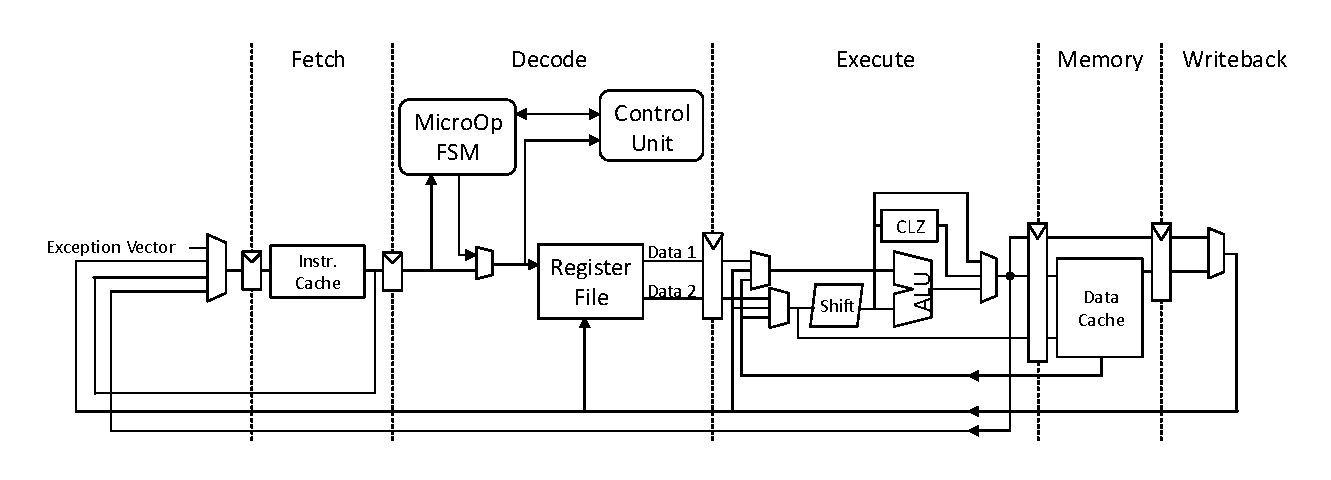
\includegraphics[width=\textwidth]{./diagrams/datapath_simple.pdf}
\caption{LEG processor core overview. More detailed diagrams are shown in the relevant sections below.}
\label{fig:core}
\end{figure}


LEG supports a subset of the ARMv5 instruction set. 
Known exceptions are the entire Thumb instruction set, LDM(2), and the rotate functionality of memory instructions.
The rotate functionality is not implemented because it appears to be unsupported in the version of qemu used to debug LEG.
All other addressing modes and instructions are supported, and any bugs that are discovered can be reported to the corresponding authors listed on the first page of this document.

The processor core is split into three main components.
The datapath contains the register file and hardware to execute arithmetic and memory operations, the controller sets multiplexers and other datapath control signals to create the specific behavior of each instruction, and the hazard unit detects dependencies between instructions and stalls the pipeline to resolve them.
A simplified overview of the processor core is summarized in Figure \ref{fig:core}.
More information about these subsystems can be found in later sections.
The datapath is described in Section \ref{sec:dp}, the controller in Section \ref{sec:c} and the hazard unit in Section \ref{sec:h}.




\subsection{Memory System}

\subsection{Core and Memory Integration}

\subsection{Exception and Interrupt Handler}

The LEG interrupt handler supports all exception types and privileged modes with the Base Restored Abort Model.
The interrupt handler is implemented as a finite state machine in \texttt{leg\_pipelined/exception\_handler.sv}.
This state machine stalls the correct pipeline stages and controls the datapath to branch to the corresponding exception vector.
More information about the exception handler can be found in Section \ref{sec:exh}


\section{Datapath}
\label{sec:dp}
The datapath

\subsection{Relevant Files}

\subsection{Fetch Stage}

\subsection{Decode Stage}

\subsection{Execute Stage}

\subsection{Memory Stage}

\subsection{Writeback Stage}

\section{Controller}
The controller

\subsection{Relevant Files}

\subsection{Decode}

\subsection{CPSR and Flags}

\subsection{MicroOp State Machine}

\section{Hazard Unit}
Hazard Unit

\subsection{Relevant Files}

\subsection{Stalls}

\subsection{Flushes}

\section{Exception Handler}
Exception Handler

\subsection{Relevant Files}

\subsection{Exception Issue State Machine}

\subsubsection{Integration to core}

\subsection{Exception Behavior}

\subsubsection{IRQ}

\subsubsection{etc}


\section{Subsystems}
% diagram
% intro
% relevant files
% technical details
\subsection{My Subsystem}

Include image

Then introduction

\subsubsection{Relevant files}
\begin{tabular}{|l|l|l|l|}
\hline File  & Description & inputs & outputs \\ 
\hline  &  &  &  \\ 
\hline  &  &  &  \\ 
\hline 
\end{tabular} 

OR 

\begin{itemize}
\item \textbf{File 1} description
\item \textbf{File 2} description
\end{itemize}

\subsubsection{Details}
\pagebreak

% TODO
\section{Data Cache}
This section describes the structure of the data cache and its role in the memory system.

\subsection{Brief Overview}

The data cache is a writeback, 2 way associative cache. 
The cache uses physical tagging and virtual indexing, so the number of bytes in each way is limited to the size of a tiny translation page (1024 bytes). 
The default cache size is $64 \text{ lines} \cdot 4 \text{ words/line} \cdot 4 \text{ bytes/word} = 1024 \text{ bytes}$. 
The number of lines per way is parameterized, and the replacement policy implemented is Least Recently Used (LRU).

\subsection{Important Diagrams}

	Figure \ref{fig:dcachediag} includes a diagram of the data cache.
	See the filed for more information.
	\begin{figure}
	\label{fig:dcachediag}
	\centering
	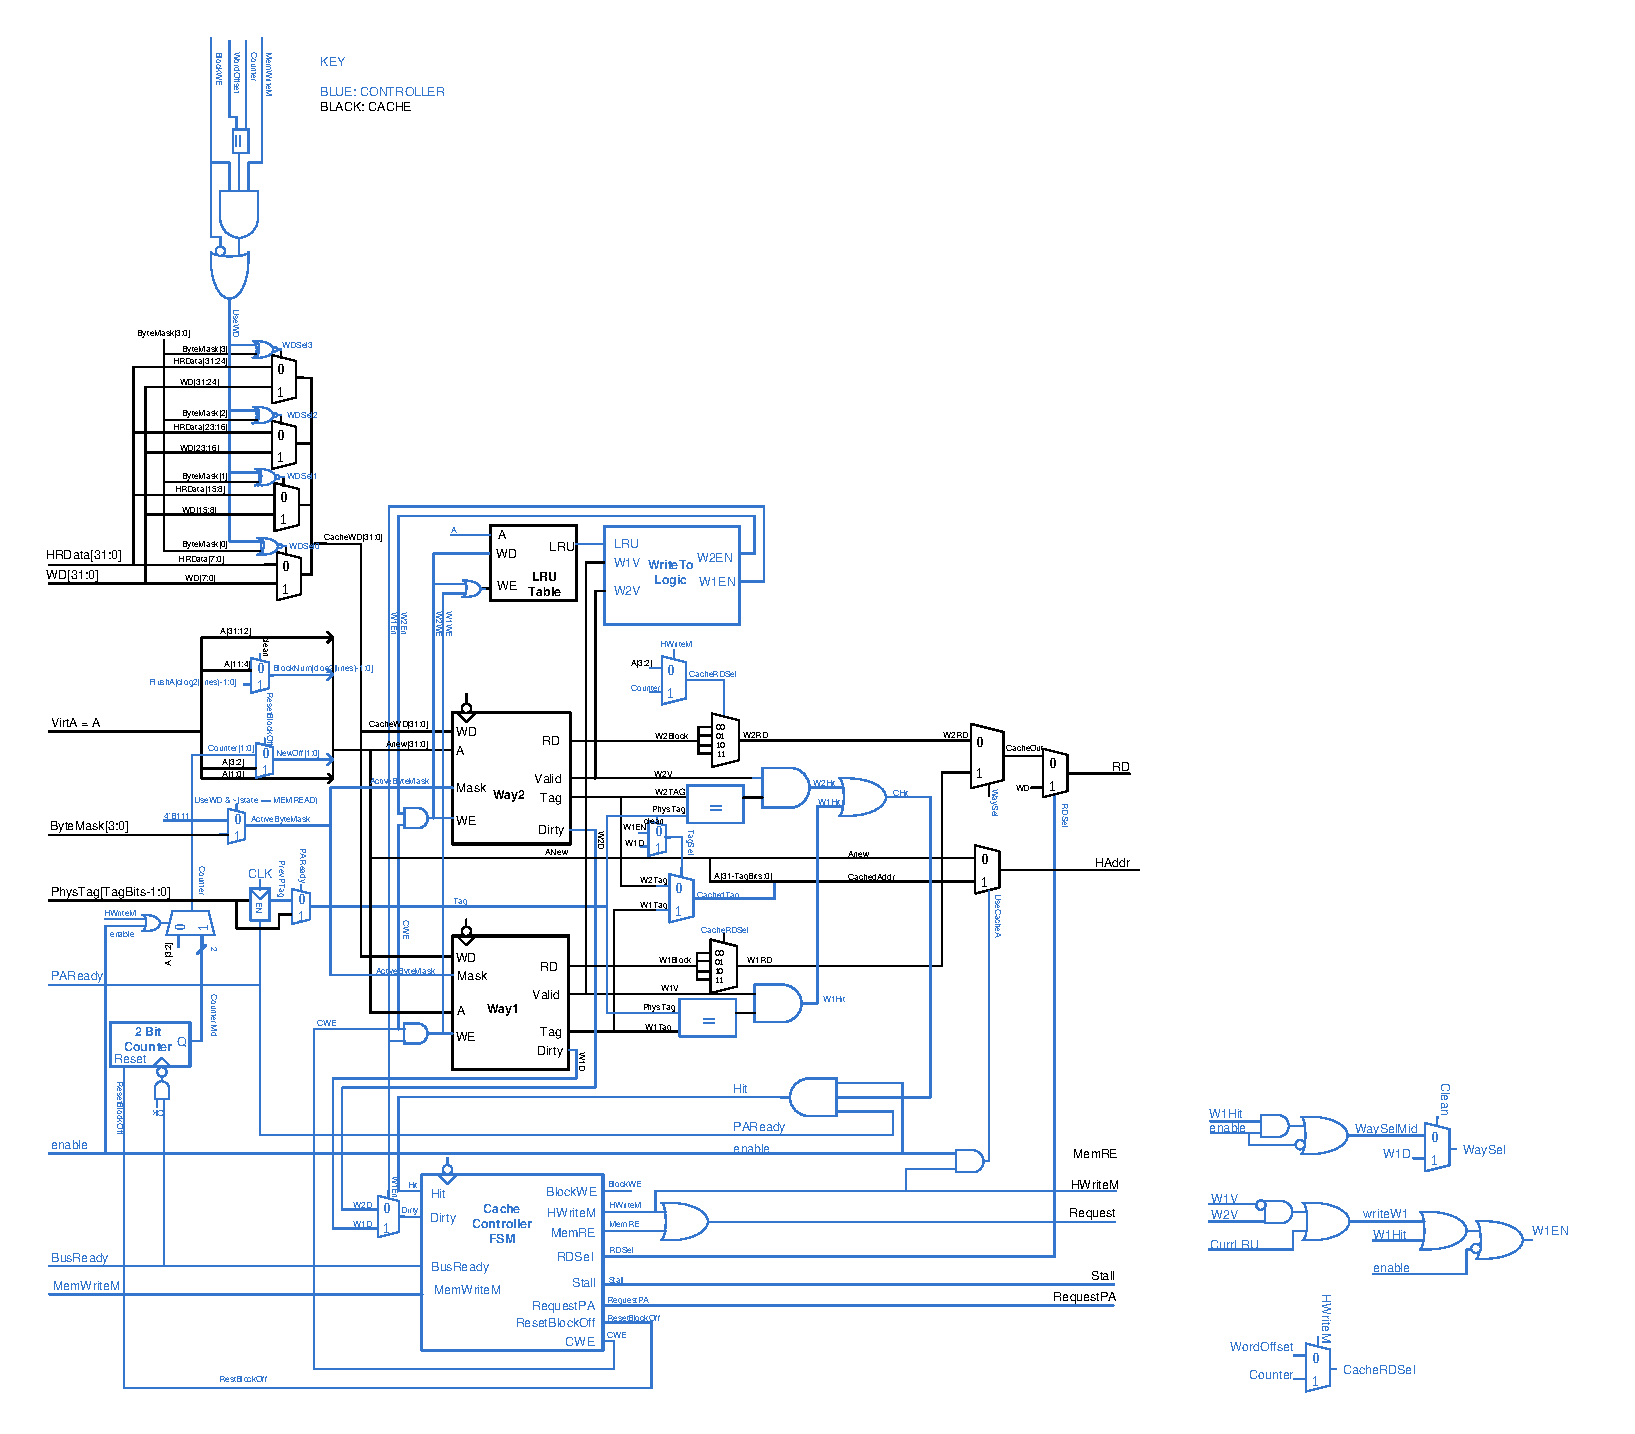
\includegraphics[width=\textwidth]{images/dataCache.pdf}
	\caption{Diagram of 2 way set associative data cache. Controller logic in blue}
	\end{figure}

% TODO - include images or give path to images in git

\subsection{All Relevant Files and Brief Descriptions}

	Table \ref{table:drel} shows the files that are used by the data cache and Table \ref{table:drel} lists the top level inputs and outputs.

	\begin{tabular}{|l|p{70mm}|}
	\hline File  & Description \\ 
	\hline  data\_writeback\_associative\_cache.sv & Top level D\$ module \\ 
	\hline  data\_writeback\_controller.sv & Controller logic for the D\$.
	Contains the primary state machine described in section \ref{sec:dstate} \\ 
	\hline  data\_writeback\_associative\_memory.sv & 
	Memory module containing the both cache ways, the LRU memory, and way selection mux's.
	This module is used in both the instruction and data caches.
	The instruction cache fixes the dirty and clean inputs to zero, because it is a read only cache.\\ 
	\hline  data\_writeback\_associative\_cache\_way.sv & 
	Contains the memory associated with one cache way. This includes four words per line along with the valid, dirty, and tag bits. \\ 
	\hline  word\_memory.sv & Byte addressable word memory  \\
	\hline
	\end{tabular} 
	\label{table:drel}
	% TODO: add caption to this table
	% \caption{Data cache files}

	\begin{tabular}{|l|p{60mm}|l|}
	\hline Port & Description & Input/Output \\ 
	\hline clk & Clock input &  I \\ 
	\hline reset & Global reset signal &  I \\ 
	\hline MemWriteM & Write signal from datapath &  I \\ 
	\hline  &  &  \\ 
	\hline
	\end{tabular} 
	\label{table:dio}
	% TODO: Add caption to this table
	% \caption{Inputs and Outputs to data cache (data\_writeback\_associative\_cache.sv)}

\subsection{Data Cache State}
\label{sec:dstate}

Below is an explanation of the states NEXTINSTR, WRITEBYTES, WAIT,and DWRITE.

\begin{enumerate}
	\item NEXTINSTR
	The next instr state removes the stall on the pipeline and allows the instructions to move one stage down the pipeline. If this stage did not exist, then the instruction at the data stage would remain the same and after the requested data is retrieved, the same data would be retrieved again. If the entry were uncachable, then the processor would stall forever.

	\item WRITEBYTES
	The cache enters this state when the cache is disabled, and it needs to writeback bytes of data. In this state, the data from the memory has been loaded into the cache and the proper bytes have been written to the cache memory. After this state, the data is stored back into the main memory with the proper bytes overwritten. This state is separate from DWRITE because writing a whole word to memory does not require loading the word first. This state will be removed when a bytemask is added to the bus.

	\item WAIT
	The data cache enters this state when simultaneous data and instruction stalls occur. The data cache has bus precedence, so it waits for the instruction cache to retrieve data before handling the next request. 

	\item DWRITE
	This state handles disables full word writes to main memory.
	
\end{enumerate}

\subsection{Not complete}

\begin{enumerate}
	\item Add Byte Mask to the ahb bus
	\item Fix the infinite loop bug at linux simulation time ~1772200
\end{enumerate}
\pagebreak

% TODO
\section{Name of thing that I made}

\subsection{Brief Overview}

% TODO

\subsection{Important Diagrams}

% TODO - include images or give path to images in git

\subsection{All Relevant Files and Brief Descriptions}

% TODO

\subsection{Analysis of Confusing Sections of Code}

% TODO
\pagebreak



\end{document}
